\section{EXPERIMENTAL RESULTS}
\label{sec:results}

The performance of the SafeSurf system has been evaluated using several key machine-learning metrics, including accuracy, precision, recall, and F1-score. 

\subsection{Dataset Description}
The system was trained and tested on the \textbf{PhiUSIIL dataset} \cite{ref10}, a comprehensive collection of over 200,000 legitimate and phishing URLs. This dataset provides a diverse range of features including lexical, network-based, and server-side attributes. To ensure execution efficiency for the real-time browser extension, the backend feature extraction logic is divided into lexical (Layer A) and infrastructure (Layer B) processing tiers.

\subsection{111-Attribute Feature Architecture}
Unlike traditional heuristic models, SafeSurf evaluates a massive 111-feature numeric array for every unique URL submission. The complete extraction pipeline natively evaluates unique occurrences spanning 17 identical special characters (e.g., \$, \&, !) rigorously computed across isolated string subsets (URL, domain, directory, file, and parameters). Table \ref{tab:features} highlights the most significant attributes driving the prediction engine.

\begin{table}[ht]
    \centering
    \caption{Selected Key Attributes for Phishing Detection}
    \label{tab:features}
    \renewcommand{\arraystretch}{1.3}
    \begin{tabular}{|p{2.5cm}|p{5cm}|}
    \hline
    \textbf{Feature Group} & \textbf{Predictive Importance} \\
    \hline
    URL / Domain Length & Masking unauthorized redirects through excessively long strings. \\
    \hline
    Lexical Frequencies & Detecting typosquatting and subdomain nesting using character counts (., -, @). \\
    \hline
    IP Implementation & Boolean indicator for raw IPv4/IPv6 addresses, common in malicious hosting. \\
    \hline
    DNS Architecture & Absence of MX/SMTP records often correlates with transient phishing setups. \\
    \hline
    Domain Lifecycle & WHOIS age; domains registered within 30-60 days have higher risk profiles. \\
    \hline
    SSL/TLS Integrity & Validating encryption chain parameters to detect server-side spoofing. \\
    \hline
    \end{tabular}
\end{table}

\subsection{Performance Metrics}
The system's classification accuracy is summarized in Table \ref{tab:test_results}. 

\begin{table}[ht]
    \centering
    \caption{Performance Summary of SafeSurf}
    \renewcommand{\arraystretch}{1.3}
  \begin{tabular}{|p{3cm}|p{3cm}|}
    \hline
    \textbf{Metric} & \textbf{Score} \\
    \hline
    Accuracy & 97.35\% \\
    \hline
    Precision & 96.80\% \\
    \hline
    Recall & 96.50\% \\
    \hline
    F1 Score & 96.65\% \\
    \hline
    ROC-AUC & 0.996 \\
    \hline
    \end{tabular}
    \label{tab:test_results}
\end{table}

The results show that SafeSurf achieved an accuracy of \textbf{97.35\%}, significantly outperforming standalone machine learning models. The classification performance is visually summarized in the confusion matrix shown in Figure \ref{fig:confusion_matrix}. Furthermore, the high ROC-AUC score of 0.996, illustrated by the ROC curve in Figure \ref{fig:roc_curve}, confirm the robustness of the system in distinguishing between legitimate and malicious websites.

\begin{figure}[htbp]
    \centering
    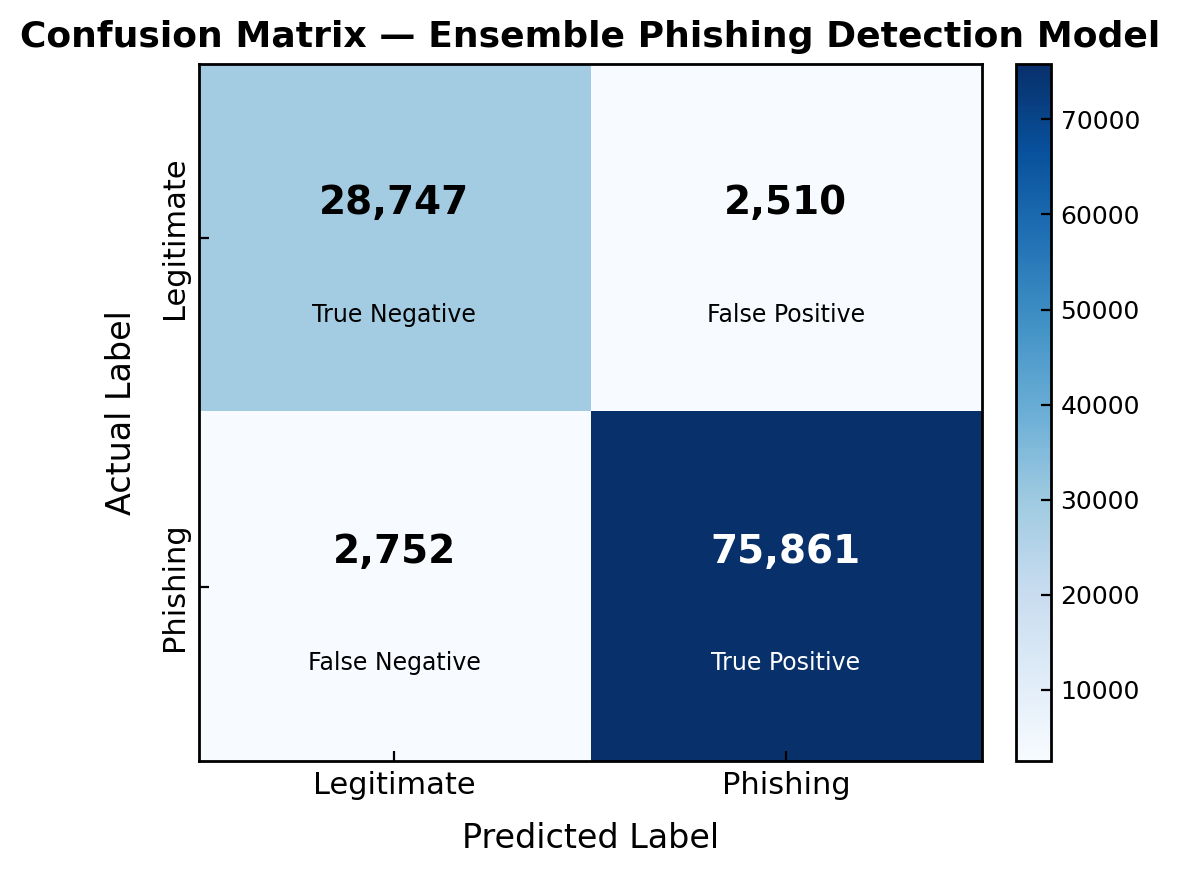
\includegraphics[width=\linewidth]{images/confusion_matrix.png}
    \caption{Confusion Matrix showing classification performance on the test set.}
    \label{fig:confusion_matrix}
\end{figure}

\begin{figure}[htbp]
    \centering
    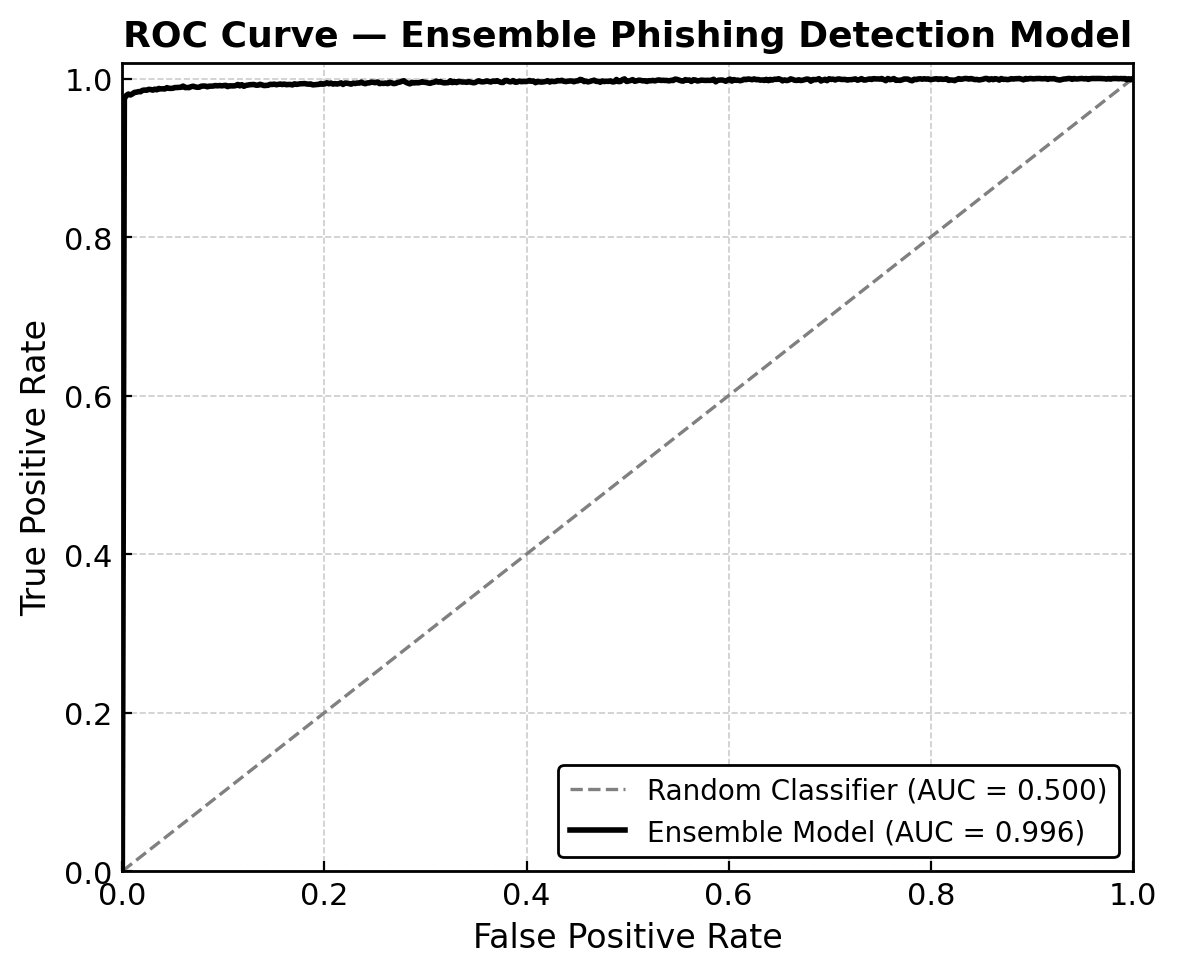
\includegraphics[width=\linewidth]{images/roc_curve.png}
    \caption{ROC Curve demonstrating the robustness of the VotingClassifier ensemble.}
    \label{fig:roc_curve}
\end{figure}

\subsection{Comparative Analysis}
SafeSurf's ensemble approach effectively identifies phishing threats that single-model classifiers would miss. By providing a layered architecture, the system maintains a high classification accuracy even against rapidly evolving and zero-day threats, outperforming various state-of-the-art detection methodologies \cite{ref3}. A multi-metric comparison of SafeSurf against baseline single-model classifiers is presented in Figure \ref{fig:performance-comparison}.

\begin{figure}[htbp]
    \centering
    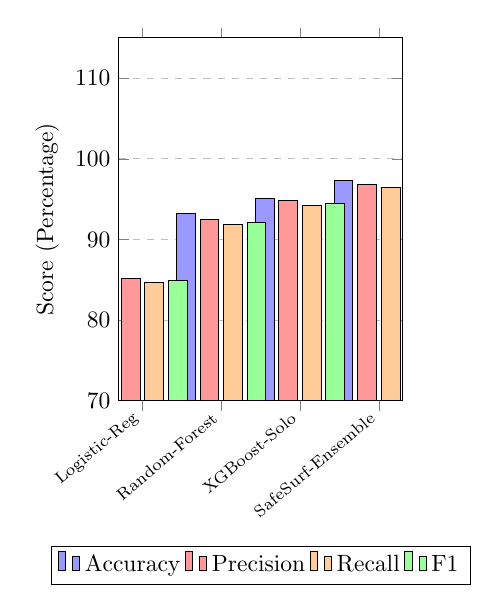
\begin{tikzpicture}[scale=0.85]
        \begin{axis}[
            ybar,
            width=0.48\textwidth,
            height=7cm,
            ylabel={Score (Percentage)},
            symbolic x coords={Logistic-Reg, Random-Forest, XGBoost-Solo, SafeSurf-Ensemble},
            xtick={Logistic-Reg, Random-Forest, XGBoost-Solo, SafeSurf-Ensemble},
            xticklabel style={rotate=40, anchor=east, font=\scriptsize},
            ymin=70, ymax=115,
            bar width=8pt,
            legend style={at={(0.5,-0.4)}, anchor=north, legend columns=-1},
            ymajorgrids=true,
            grid style=dashed,
        ]
            \addplot[fill=blue!40] coordinates {
                (Logistic-Reg,86.4) (Random-Forest,93.2) (XGBoost-Solo,95.1) (SafeSurf-Ensemble,97.35)
            };
            \addplot[fill=red!40] coordinates {
                (Logistic-Reg,85.1) (Random-Forest,92.5) (XGBoost-Solo,94.8) (SafeSurf-Ensemble,96.80)
            };
            \addplot[fill=orange!40] coordinates {
                (Logistic-Reg,84.7) (Random-Forest,91.8) (XGBoost-Solo,94.2) (SafeSurf-Ensemble,96.50)
            };
            \addplot[fill=green!40] coordinates {
                (Logistic-Reg,84.9) (Random-Forest,92.1) (XGBoost-Solo,94.5) (SafeSurf-Ensemble,96.65)
            };
            \legend{Accuracy, Precision, Recall, F1}
        \end{axis}
    \end{tikzpicture}
    \caption{Performance Comparison Against Baseline Models (Multi-Metric Analysis)}
    \label{fig:performance-comparison}
\end{figure}
